
\documentclass[12pt,letter]{article}

\usepackage{titlesec}
\usepackage[top=0.75in,bottom=0.75in,left=0.75in,right=0.75in]{geometry}

\titleformat{\subsubsection}[runin]{\normalfont\large\bfseries}{\thesubsubsection}{1em}{}

\usepackage{amsmath,mathrsfs, textcomp}
\usepackage{amssymb}
\usepackage{pstricks,pst-plot,psfrag}
\usepackage[all]{xy}
\usepackage{graphicx,subfigure,xspace,bm}
\usepackage[retainorgcmds]{IEEEtrantools}
\graphicspath{ {images/}}
% Commands for algorithms
%\usepackage{algorithm,algorithmic}
\usepackage[lined,linesnumbered,algoruled,noend]{algorithm2e}
\usepackage{float} 
 
\newtheorem{theorem}{Theorem}
\newtheorem{definition}{Definition}
\newtheorem{assumption}[theorem]{Assumption}
\newtheorem{lemma}{Lemma}
\newtheorem{claim}[theorem]{Claim}
\newtheorem{remarks}[theorem]{Remarks}
\newtheorem{remark}[theorem]{Remark}
\newtheorem{example}[theorem]{Example}
\newtheorem{corollary}[theorem]{Corollary}
\newtheorem{proposition}[theorem]{Proposition}  

\newcommand{\theoremautorefname}{Theorem}
\newcommand{\definitionautorefname}{Definition}
\newcommand{\lemmaautorefname}{Lemma}
\newcommand{\remarkautorefname}{Remark}
\newcommand{\propositionautorefname}{Proposition}
\newcommand{\exampleautorefname}{Example}

%
\newtheorem{proof}[theorem]{Proof}
\newcommand{\qed}{\hfill $\blacksquare$}

\newcommand{\longthmtitle}[1]{\mbox{}\textup{\textbf{(#1):}}}


% GENERAL NOTATIONS
\newcommand{\real}{{\mathbb{R}}}
\newcommand{\complex}{{\mathbb{C}}}
\newcommand{\realpart}{\mathrm{Re}}
\newcommand{\impart}{\mathrm{Im}}
\newcommand{\realpositive}{{\mathbb{R}}_{>0}}
\newcommand{\realnonnegative}{{\mathbb{R}}_{\ge 0}}
\newcommand{\integers}{\mathbb{Z}}
\newcommand{\integerp}{\mathbb{Z}_{\geq 1}}
\newcommand{\eps}{\epsilon}
\newcommand{\argmin}{\operatorname{argmin}}
\newcommand{\until}[1]{\{1,\dots,#1\}}
\newcommand{\map}[3]{#1:#2 \rightarrow #3}
\newcommand{\setmap}[3]{#1:#2 \rightrightarrows #3}
\newcommand{\equilibria}[1]{\operatorname{Eq}(#1)}
\newcommand{\pder}[2]{\frac{\partial #1}{\partial #2}}
\newcommand{\pdertwo}[2]{\frac{\partial^2 #1}{\partial #2^2}}
\newcommand{\pdertwom}[3]{\frac{\partial^2 #1}{\partial #2\partial #3}}
 \newcommand{\adve}{\subscr{\Sigma}{adv}}
\newcommand{\Alin}{A_{\mathrm{linear}}}
\renewcommand{\Alin}{A}
\newcommand\subscr[2]{#1_{\textup{#2}}}
\newcommand\upscr[2]{#1^{\textup{#2}}}
\newcommand\upsubscr[3]{#1_{\textup{#2}}^{\textup{#3}}}
\newcommand{\TwoNorm}[1]{\|#1\|_2}
\newcommand{\argmax}{\mathrm{argmax}}


%% Enumerate environment
\renewcommand{\theenumi}{(\roman{enumi})}
\renewcommand{\labelenumi}{\theenumi}
\newcommand{\margin}[1]{\marginpar{\color{red}\tiny\ttfamily#1}}
\newcommand{\marginb}[1]{\marginpar{\color{blue}\tiny\ttfamily#1}}
\newcommand{\bah}[1]{{\color{blue} #1}}


% NEW
\newcommand{\diag}{\mathrm{diag}}
%%%
% Numbers on top

%\parskip = .25ex
%\renewcommand{\baselinestretch}{1.45}

\newcommand{\myclearpage}{\clearpage}
 \renewcommand{\myclearpage}{}
\usepackage[hidelinks]{hyperref}
 \usepackage[T1]{fontenc}
 \usepackage[osf]{mathpazo}
 \usepackage{wrapfig}
\usepackage{mathptmx}

\usepackage{xcolor}
\usepackage{pagecolor}
\usepackage{lipsum}  

%\pagecolor{black}
%\color{white}

 \definecolor{BBlue}{cmyk}{.98,0.10,0,.25}

\def\doubleunderline#1{\underline{\underline{#1}}}

\newcommand{\myemph}[1]{\textcolor{BBlue}{\textbf{#1}}}
\usepackage{fancyhdr}
\pagestyle{fancyplain}
\rhead{Himesh Bhatia}

\begin{document}
\bstctlcite{IEEEexample:BSTcontrol}
\title{\vspace{-4ex} Neural Networks \vspace{-4ex}}
\author{}
\date{}
\maketitle

Neural networks consist of either neurons or perceptrons that are connected in a series
of layers.
These neural networks are models of the human brain, which consists of trillions of neurons
that fire together. 
In order to understand neural networks, we first have to ask what is a perceptron and a neuron.

\section{Perceptrons and Neurons}
\subsection{Perceptrons}
Perceptrons have several inputs and produces a binary output. 
Let $\mathbb{X} \subseteq \real$ be the space of input signals, 
and $\mathbb{Y} \subseteq \real$ be the space of output signals. 
Suppose a perceptron has $n$ inputs,  $\{x_k\}_{k=1}^{n}$. 
Each input has an associated weight,
$\{w_k\}_{k=1}^{n} \subset \real$.
Then the output of the perceptron, $y$, is defined as 
\begin{IEEEeqnarray*}{rCl}
	y &=& 
	\begin{cases}
		1 & \text{if } \displaystyle{\sum_{k = 1}^n {x_{k} w_{k}}> t},\\
		0 & \text{if } \displaystyle{\sum_{k = 1}^n {x_{k} w_{k}} \leq t},
	\end{cases}
\end{IEEEeqnarray*}
where $t \in \real$ is the defined as the threshold of the perceptron. 
However, having the output as either a $0$ or $1$ is restrictive, so we can expand the 
model of the perceptron to a neuron.

\subsection{Neurons}
Neurons also take several inputs, but instead of producing a binary output, it produces
a real number between $[0, 1]$. 
Suppose a neuron has $n$ inputs,  $\{x_k\}_{k=1}^{n}$. 
Each input has an associated weight,
$\{w_k\}_{k=1}^{n} \subset \real$. 
The neuron has an associated bias $b \in \real$.
Define a sigmoid function $\sigma : \real \rightarrow [0,1]$ as a $C^{1}[0,1]$ function.
Then the output or \textit{activation} is 
\begin{IEEEeqnarray*}{rCl}
	y &=& \sigma \left ( \sum^{n}_{k = 1} {x_{k} w_{k}} + b \right ) 
\end{IEEEeqnarray*}
It is important to choose a $C^{1}[0,1]$ function as the sigmoid function 
because the derivative of the sigmoid function is used 
in the equations of backpropagation. 
Examples of sigmoid functions are $\sigma(x) = \tanh(x)$ or 
$\sigma(x) = \frac{1}{1+e^{-x}}$. 

\begin{figure}[h]
	\caption{An example of a neuron}
	\centering
	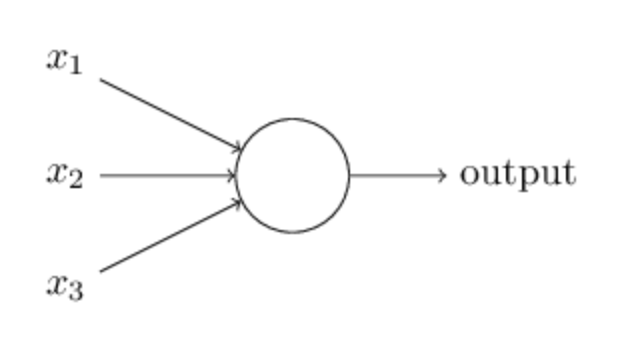
\includegraphics[scale=0.65]{perceptrons}
\end{figure}

\section{Neural networks}
Neural networks have several layers of neurons whose inputs come from the previous layer. 
Let $\mathbb{X} \subseteq \real^{n}$ be the input space, 
$\mathbb{Y} \subseteq \real^{m}$ be the output space,
and suppose we have $k$ layers in our network.
In each layer, we have $l_{i} \in \integers_{>0}$ neurons, $i \in \{1, \ldots, k \}$, where 
the $1^{st}$ layer is the input layer,
and $k^{th}$ layer is the output layer. 

Let $\alpha_{i}^{j}$ be the activation of the $i^{th}$ neuron in the 
$j^{th} \in \{2, \ldots, k\}$ layer. 
Let us define $w_{h, i}^{j} \in \real$ be the weight of the connection from 
the $h^{th}$ neuron from the $(j-1)^{th}$
layer to the $i^{th}$ neuron in the $j^{th}$ layer.
Let $b_{i}^{j} \in \real$ be the bias associated with the $i^{th}$ neuron in the $j^{th}$ layer. 
Then the activation of the neuron is  
\begin{IEEEeqnarray}{rCl} \label{actEqn}
	\alpha_{i}^{j} &=& \sigma \left ( \sum_{h = 1}^{l_{j-1}} 
	w_{h, i}^{j} \alpha_{h}^{j-1} + b_{i}^{j}\right )
\end{IEEEeqnarray}

Note that we can simplify these definitions by using vectors and matrices. 
Let \underbar{$\alpha^{j}$} $= \left (\alpha_{1}^{j}, \ldots, \alpha_{l_{j}}^{j} \right)^{T}$ 
be the activation vector of the $j^{th}$ layer.
Let \doubleunderline{$W^{j}$}$ = \left[w_{h, i}^{j} \right]_{h, i}^{T}$ 
be the matrix of the weights of the connections from the $(j-1)^{th}$ to the $j^{th}$ layer. 
Let \underline{$b^{j}$} $ = \left (b_{1}^{j}, \ldots, b_{l_{j}}^{j} \right)^{T}$ 
be the bias vector of the $j^{th}$ layer. 
Then equation \ref{actEqn} becomes
\begin{IEEEeqnarray*}{rCl}
	\text{\underline{$\alpha^{j}$}} &=& \sigma \left ( 
	\text{\doubleunderline{$W^{j}$}}  \ 
	\text{\underline{$\alpha^{j-1}$}} + \text{\underline{$b^{j}$}} \right)
\end{IEEEeqnarray*}

Remark that we set \underline{$\alpha^{1}$} $ = $ \underline{$x$}, where \underline{$x$} 
$\in \real^{n}$ is the input vector. 
We will also denote 
$$z_{i}^{j} = \sum_{h = 1}^{l_{j-1}} w_{h, i}^{j} \alpha_{h}^{j-1} + b_{i}^{j} $$

When constructing a neural network, the weights and the biases are the parameters
that can be fine tuned to optimize the neural network. 
I have several ideas to find the optimal parameters, 
specifically the idea that we try to apply Bayesian analysis or control theory. 
We could also try to use Fourier analysis. 
However, to proceed, we need to define how well the neural network performs. 
For this, we need to define a cost function. 

Let \underline{$a$} $\in \mathbb{Y}$ be the desired output for some given input \underline{$x$}. 
We have call $($\underline{$x$} $,$ \underline{$a$}$)$ the \textit{training data} for the 
neural network.  
Then the \textit{cost function} is defined as 
$$C:\mathbb{Y} \times \mathbb{Y} \rightarrow \real_{\geq 0}$$
Generally, we will use the squared error:
$$C(\text{\underbar{$a$}, \underbar{$y$}}) = \| \text{\underbar{$a$} $-$ \underbar{$y$}} \|_{2}$$
or the cross-entropy function:
$$C(\text{\underbar{$a$}, \underbar{$y$}}) = -\sum_{j = 1}^{m}  a_{m} \ln(y_{m}) \
+ (1-a_{m}) \ln(1-y_{m})$$


\subsection{Backpropagation equations}
The aim of backpropagation equations is to find $\frac{\partial C}{\partial w_{h, i}^{j}}$
and $\frac{\partial C}{\partial b_{j}^{j}}$ so we can minimize the cost function 
with the parameters we can control.
We can do this indirectly by first calculating 
$\delta_{i}^{j} = \frac{\partial C}{\partial z_{i}^{j}}$ and related to what we want. 
Let us first calculate this for the output layer (the $k^{th}$ layer).
Note that $y_{j} = \sigma \left( z_{j}^{k} \right)$ and hence 
\begin{IEEEeqnarray*}{rCl}
	\frac{\partial y_{j}}{\partial z_{i}^{k}} = 
	\begin{cases}
		\sigma^{'} \left( z_{j}^{k} \right) & \text{if } j = i, \\
		0 & \text{otherwise}
	\end{cases}
\end{IEEEeqnarray*}
Thus, we have
\begin{IEEEeqnarray*}{rCl} \label{backprop1}
	\delta_{i}^{k} &=& \frac{\partial C}{\partial z_{i}^{k}} \\
	\delta_{i}^{k} &=& \sum_{j=1}^{m} \frac{\partial C}{\partial y_{j}} 
	\frac{\partial y_{j}}{\partial z_{i}^{k}} \\
	\delta_{i}^{k} &=& \frac{\partial C}{\partial y_{i}}
	\sigma^{'} \left( z_{i}^{k} \right) \IEEEyesnumber
\end{IEEEeqnarray*}

Using this, we can find $\delta_{i}^{j} = \frac{\partial C}{\partial z_{i}^{j}}$ for any
$j \in \{ 1, \ldots, k-1 \}$.  
Note that,
\begin{IEEEeqnarray*}{rCl}
	z_{p}^{j+1} &=& \sum_{h = 1}^{l_{j}} w_{h, p}^{j+1} \alpha_{h}^{j} + b_{p}^{j+1} \\
	z_{p}^{j+1} &=& \sum_{h = 1}^{l_{j}} w_{h, p}^{j+1} 
	\sigma \left (z_{h}^{j} \right) + b_{p}^{j+1} \\
	\Rightarrow \frac{\partial z_{p}^{j+1}}{\partial z_{i}^{j}} 
	&=& w_{i, p}^{j+1} \sigma^{'} \left ( z_{i}^{j} \right)
\end{IEEEeqnarray*}
where $z_{h}^{1} = x_{h}$. 
Hence,
\begin{IEEEeqnarray*}{rCl} \label{backprop2}
	\delta_{i}^{j} &=& \frac{\partial C}{\partial z_{i}^{j}} \\
	\delta_{i}^{j} &=& \sum_{p=1}^{m} \frac{\partial C}{\partial z_{p}^{j+1}}
	\frac{\partial z_{p}^{j+1}}{\partial z_{i}^{j}} \\
	\delta_{i}^{j} &=& \sum_{p=1}^{m} \delta_{p}^{j+1} 
	w_{i, p}^{j+1} \sigma^{'} \left ( z_{i}^{j} \right) \IEEEyesnumber
\end{IEEEeqnarray*}

We can related equations \ref{backprop1} and \ref{backprop2}
to find $\frac{\partial C}{\partial w_{h, i}^{j}}$
and  $\frac{\partial C}{\partial b_{i}^{j}}$.
That is
\begin{IEEEeqnarray*}{rCl} \label{backprop3}
	\delta_{i}^{j} &=& \frac{\partial C}{\partial z_{i}^{j}} \\
	\delta_{i}^{j} &=& \frac{\partial C}{\partial b_{i}^{j}} 
	\frac{\partial b_{i}^{j}}{\partial z_{i}^{j}} \\
	\delta_{i}^{j} &=& \frac{\partial C}{\partial b_{i}^{j}} \IEEEyesnumber
\end{IEEEeqnarray*}
and
\begin{IEEEeqnarray*}{rCl} \label{backprop4}
	\frac{\partial C}{\partial w_{h, i}^{j}} &=& \sum_{p = 1}^{l_{j}} 
	\frac{\partial C}{\partial z_{p}^{j}} 
	\frac{\partial z_{p}^{j}}{\partial w_{h, i}^{j}} \\
	\frac{\partial C}{\partial w_{h, i}^{j}} &=& \frac{\partial C}{\partial z_{h}^{j}}
	\frac{\partial z_{h}^{j}}{\partial w_{h, i}^{j}} \\
	\frac{\partial C}{\partial w_{h, i}^{j}} &=& \delta_{h}^{j} \alpha_{i}^{j-1} 
	\IEEEyesnumber
\end{IEEEeqnarray*}



\end{document}
